\documentclass[12pt,a4paper]{article}
\usepackage{lmodern}
\usepackage{amssymb,amsmath}
\usepackage{ifxetex,ifluatex}
\usepackage{fixltx2e} % provides \textsubscript
\ifnum 0\ifxetex 1\fi\ifluatex 1\fi=0 % if pdftex
  \usepackage[T1]{fontenc}
  \usepackage[utf8]{inputenc}
\else % if luatex or xelatex
  \ifxetex
    \usepackage{mathspec}
  \else
    \usepackage{fontspec}
  \fi
  \defaultfontfeatures{Ligatures=TeX,Scale=MatchLowercase}
\fi
% use upquote if available, for straight quotes in verbatim environments
\IfFileExists{upquote.sty}{\usepackage{upquote}}{}
% use microtype if available
\IfFileExists{microtype.sty}{%
\usepackage{microtype}
\UseMicrotypeSet[protrusion]{basicmath} % disable protrusion for tt fonts
}{}
\usepackage[margin=2cm]{geometry}
\usepackage{hyperref}
\hypersetup{unicode=true,
            pdftitle={A proposed approach to estimating excess mortality associated with cleft lip / cleft palate},
            pdfauthor={Mark Myatt},
            pdfborder={0 0 0},
            breaklinks=true}
\urlstyle{same}  % don't use monospace font for urls
\usepackage{graphicx,grffile}
\makeatletter
\def\maxwidth{\ifdim\Gin@nat@width>\linewidth\linewidth\else\Gin@nat@width\fi}
\def\maxheight{\ifdim\Gin@nat@height>\textheight\textheight\else\Gin@nat@height\fi}
\makeatother
% Scale images if necessary, so that they will not overflow the page
% margins by default, and it is still possible to overwrite the defaults
% using explicit options in \includegraphics[width, height, ...]{}
\setkeys{Gin}{width=\maxwidth,height=\maxheight,keepaspectratio}
\IfFileExists{parskip.sty}{%
\usepackage{parskip}
}{% else
\setlength{\parindent}{0pt}
\setlength{\parskip}{6pt plus 2pt minus 1pt}
}
\setlength{\emergencystretch}{3em}  % prevent overfull lines
\providecommand{\tightlist}{%
  \setlength{\itemsep}{0pt}\setlength{\parskip}{0pt}}
\setcounter{secnumdepth}{0}
% Redefines (sub)paragraphs to behave more like sections
\ifx\paragraph\undefined\else
\let\oldparagraph\paragraph
\renewcommand{\paragraph}[1]{\oldparagraph{#1}\mbox{}}
\fi
\ifx\subparagraph\undefined\else
\let\oldsubparagraph\subparagraph
\renewcommand{\subparagraph}[1]{\oldsubparagraph{#1}\mbox{}}
\fi

%%% Use protect on footnotes to avoid problems with footnotes in titles
\let\rmarkdownfootnote\footnote%
\def\footnote{\protect\rmarkdownfootnote}

%%% Change title format to be more compact
\usepackage{titling}

% Create subtitle command for use in maketitle
\newcommand{\subtitle}[1]{
  \posttitle{
    \begin{center}\large#1\end{center}
    }
}

\setlength{\droptitle}{-2em}
  \title{A proposed approach to estimating excess mortality associated with cleft
lip / cleft palate}
  \pretitle{\vspace{\droptitle}\centering\huge}
  \posttitle{\par}
  \author{Mark Myatt}
  \preauthor{\centering\large\emph}
  \postauthor{\par}
  \date{}
  \predate{}\postdate{}


\begin{document}
\maketitle

This note describes a simple and cheap method that may be useful for the
estimating excess mortality associated with cleft lip / cleft palate in
settings where reporting of congenital anomalies is incomplete or
absent. It is intended as a request for comments.

The method uses:

\begin{itemize}
\item
  Readily available survey data (e.g.~census tables, DHS, MICS) or
  simple survey data that can describe the age-distribution of the
  general population.
\item
  Data on the ages of found cases from clinical settings (may suffer a
  selection bias) and from community-based case-finding exercises
  (e.g.~using active and adaptive case-finding).
\end{itemize}

The method is designed to be very low cost (i.e.~compared to a cohort
study) and to increase the impact of programs treating cleft lip / cleft
palate through the introduction or expansion of community-based
case-finding and referral.

Mortality in the general population is estimated from the population age
distribution using a simple exponential decay model in which the
proportion of the birth cohort surviving at each age follows:

~

\begin{equation}
\rho ~ = ~ e ^ {-zt}
\end{equation}

~

where \(e\) is the base of the natural logarithm (approximately 2.7183),
\(z\) is the mortality rate, and \(t\) is age. Given an age-distribution
(e.g.~as shown in Figure 1) we can fit the model:

~

\begin{equation}
log_e(n) ~ = ~ \alpha ~ + ~ \beta ~ \times ~ t
\end{equation}

~

where \(n\) is the count of children in each age group. The absolute
value of \(\beta\) is an estimate of the mortality rate (\(z\)) in the
general population. For the data shown in Figure 1 this is
\(z = 0.028205\) which is equivalent to about 0.77 / 10,000 / day. The
expected counts for the model:

~

\begin{equation}
\rho ~ = ~ e ^ {-0.028205 ~ \times ~ t}
\end{equation}

~

are shown in red in Figure 1. We can fit a similar model to the ages of
cases of cleft lip / cleft palate found in clinical data and by
community-based case-finding. Given the age distribution of cases shown
in Figure 2 we estimate \(z\) to be 0.36690 which is equivalent to about
10 / 10,000 / day.

Excess mortality can be estimated as the ratio of the two mortality
rates:

~

\begin{equation}
\text{Morality rate ratio} ~ = ~ \frac{z_\text{cases}}{z_\text{General population}}
\end{equation}

~

with the example data this is:

~

\begin{equation}
\text{Morality rate ratio} ~ = ~ \frac{0.36690}{0.028205} ~ = ~ 13.01
\end{equation}

~

Mortality in cases is about thirteen times higher than the general
population.

A 95\% confidence interval could be calculated using the bootstrap.

It is envisaged that data for children and cases aged between 6 months
and 5 years (the simple exponential decay model may not hold with older
children and adults) will be used and that age will be recorded to best
possible accuracy and precision.

\newpage

\begin{figure}

{\centering 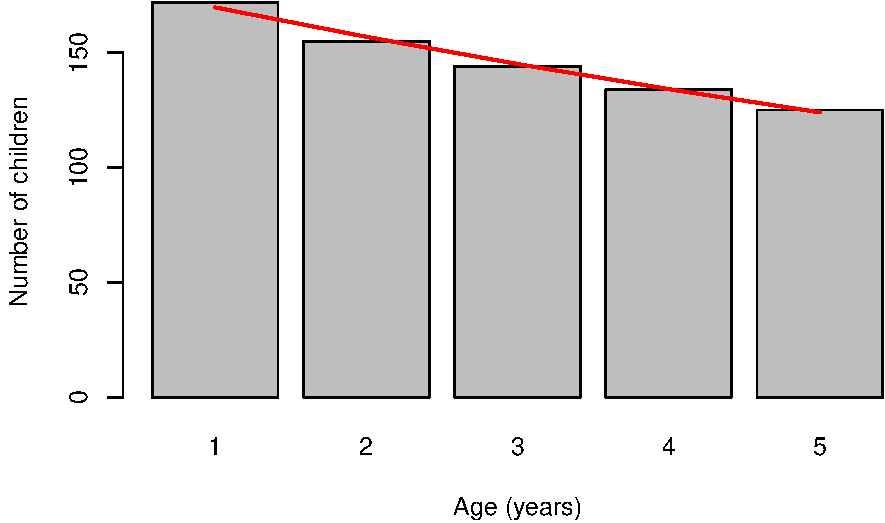
\includegraphics{figures/figure1-1} 

}

\caption{Example age distribution (0 to 5 years) in the general population}\label{fig:figure1}
\end{figure}

\begin{figure}

{\centering 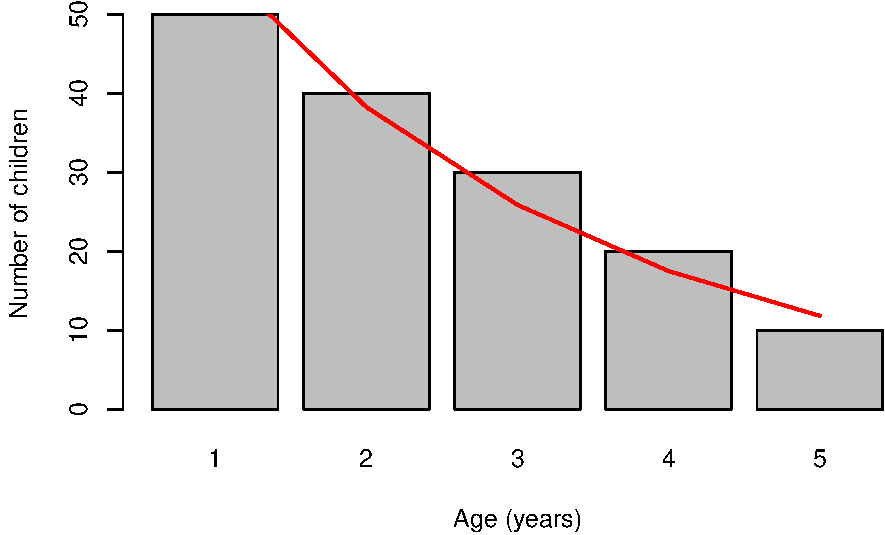
\includegraphics{figures/figure2-1} 

}

\caption{Example age distribution (0 to 5 years) in cases}\label{fig:figure2}
\end{figure}


\end{document}
